\documentclass[10pt,letterpaper,onecolumn,draftclsnofoot]{IEEEtran}
\usepackage[margin=0.75in]{geometry}
\usepackage{listings}
\usepackage{color}
\usepackage{longtable}
\usepackage{tabu}
\definecolor{dkgreen}{rgb}{0,0.6,0}
\definecolor{gray}{rgb}{0.5,0.5,0.5}
\definecolor{mauve}{rgb}{0.58,0,0.82}

\lstset{frame=tb,
  language=C,
  columns=flexible,
  numberstyle=\tiny\color{gray},
  keywordstyle=\color{blue},
  commentstyle=\color{dkgreen},
  stringstyle=\color{mauve},
  breaklines=true,
  breakatwhitespace=true,
  tabsize=4
}

\begin{document}
\begin{titlepage}
  \title{CS 444 - Spring 2016 - Final Paper}
  \author{Cody Malick\\
  \texttt{malickc@oregonstate.edu}}
  \date{June 8, 2016}
  \maketitle
  \vspace*{4cm}
  \begin{abstract}
      \noindent Understanding how an operating system functions, from handling user
      input, to managing memory, is important for any aspiring kernel developer to
      understand. In this report, a basic overview of many topics that are fundamental
      to operating system understanding are covered. Each topic is covered for Linux,
      Windows, and FreeBSD, then contrasted.


  \end{abstract}
\end{titlepage}

\tableofcontents
\clearpage
\section{Introduction}
Operating systems are complex beasts. Often they scare away developers that might
be interested in working with them simply from intimidation or lack of fondness for
C based languages. I have discovered this term that, although operating systems have many facets and complexities, many of the topics are interesting and easy to study and tweak. This paper covers many of the operating system subsystems studied this term. This includes processes, process scheduling, interrupts and interrupt handlers, memory management, and file systems.

\section{Processes and Scheduling}

\subsection{Introduction}
The first topic is that of processes and process scheduling. This section
contains descriptions on how each of the operating systems, Linux, Windows,
and FreeBSD handle processes, threads, and CPU scheduling. A lot can be
learned about the design decisions of the minds behind the operating system by
how they handle these core constructs. We will start by describing how Linux
handles these, as Linux is the focus of this class.

\subsection{Linux}
\subsubsection{Processes}
The first thing that should be defined, is simply what a process is: "A
\textit{process} is a program (object code stored on some media) in the midst of
execution."\cite{robertlove2010} Although the Linux kernel refers to processes
as tasks, in this section (for uniformity) we will only refer to them as processes.

A process in Linux is ultimately born, somewhere up the line, from the
\texttt{init} process. The \texttt{init} is the absolute root of every process
tree on any Linux machine. It has a process ID of 1. All processes are spawned
from either the \texttt{fork()} or \texttt{exec()} function calls. \texttt{Fork()}
creates an exact copy of the calling process as a child of the process, while
\texttt{exec()} loads a new executable into the process space and executes it.
These are the only ways new processes are created in Linux.

Each process has a process descriptor that describes every aspect of
the process, the \texttt{task\_struct}. The \texttt{task\_struct} is contained
in \texttt{<linux/sched.h>}. \texttt{Task\_struct} describes the current state
of the process, the parent process ID, the process ID, exit code, priority, etc.
Everything you could possibly want to know about a process in Linux is in that
struct. I've included the \texttt{Task\_struct} as Appendix A as it is a very
large structure.

Processes, of course, must have states of execution. On Linux, processes have
five states, each represented by flags in the \texttt{task\_struct}:

\begin{description}
	\item \texttt{TASK\_RUNNING}: The process is either running or in a run-queue
	ready to be run (run-queues will be discussed in the CPU scheduling section).
	\item \texttt{TASK\_INTERRUPTIBLE}: the process is sleeping (blocked) waiting
	for a condition to un-block. Once the condition is met, it transitions to
	\texttt{TASK\_RUNNING}.
	\item \texttt{TASK\_UNINTERRRUPTIBLE}: The same state as \texttt{TASK\_INTERRUPTIBLE}
	with the difference being that it does not wake once an interrupt is received.
	\item \texttt{\_TASK\_TRACED}: This flag shows that the process is being traced
	by another process. An example is GDB.
	\item \texttt{\_TASK\_STOPPED}: Process execution has halted and it is not
	possible to start running. This state is a result of a halting interrupt from
	the CPU, or if a debugger sends it a signal.
\end{description}

\subsubsection{Threads}
As with processes, we will define what a thread is: ``Threads of execution, often
shortened to \textit{threads}, are the objects of activity within the process.''
\cite{robertlove2010} In Linux, threads are treated fundamentally the same as
processes. The only difference is that they have a shared address space,
filesystem resources, file descriptors, and signal handlers. Here is the
\texttt{thread\_info} struct:\cite{robertlove2010}

\begin{lstlisting}[caption=The Linux thread\_info structure is how Linux tracks essential information about each thread and process]
struct thread_info {
	struct task_struct    *task;
	struct exec_domain    *exec_domain;
	unsigned long         flags;
	unsigned long         status;
	__u32                 cpu;
	__s32                 preempt_count;
	mm_segment_t          addr_limit;
	struct restart_block  restart_block;
	unsigned long         previous_esp;
	__u8                  supervisor_stack[0];
};
\end{lstlisting}

Compared to the \texttt{task\_struct}, this is a relatively simple data structure.
It has a pointer to the \texttt{task\_struct} that is unique to that thread,
along with a few extra flags and sets of information that separate threads from
processes.

\subsubsection{CPU Scheduling}
Linux ships with a few different schedulers by default, including a real time
scheduler.\cite{redhat2016} The default scheduler for Linux is the CFS, or
the Completely Fair Scheduler.
The CFS is only fair in so far as it tries its best to split the processors time
into equal bits, 1/n, where n is the number of processes currently running. The
CFS weights this with process priority, or nice value, and the higher the weight
the larger percentage of processor time that process gets. So it's not completely
fair, but that is the idea behind it.

One of the major problems with this system is that a very large chunk of processes
creates incredibly small slices of CPU time. For example, if there were six-thousand
processes and/or threads that all had the same weight, then the cpu slice for
each process would be 1/6000. There is a point where that slice is not large
enough to even complete the context switch required to start executing the process
again. The CFS handles this by implementing a floor on slice size, known as
\textit{minimum granularity}.\cite{robertlove2010} With this system, every process
will always have a minimum amount of run time, but the system can become very
slow once this size is reached.

% https://www.kernel.org/doc/Documentation/scheduler/sched-design-CFS.txt
% This is a good resource for indepth analysis of the scheduler

\subsection{Windows}
Windows is a very different beast. The process and thread structure are quite a
bit different from Linux. The CPU scheduler Windows uses has the same basic idea
as the CFS, but varies greatly when it comes to how it handles priority and division
of CPU time.
\subsubsection{Processes}
Processes in Windows are similar to Linux in only one way: the both have a
process ID. Otherwise, processes in Windows handle very differently than Linux.
Here is the basic process struct in Windows, \texttt{\_PROCESS\_INFORMATION}:
\cite{msprocstruct2016}

\begin{lstlisting}[caption=The Windows \_PROCESS\_INFORMATION Structure is how Windows
tracks some important information about each thread and process]
typedef struct _PROCESS_INFORMATION {
	HANDLE hProcess;
	HANDLE hThread;
	DWORD  dwProcessId;
	DWORD  dwThreadId;
} PROCESS_INFORMATION, *LPPROCESS_INFORMATION;
\end{lstlisting}

The \texttt{HANDLE} data type is a 32-bit unique identifier stored in the Windows
kernel to identify individual processes.\cite{mshandle2016} The \texttt{hThread}
points to the primary thread a process is executing on. These first two of these
identifying fields are used internally by the kernel to specify what functions
are performing operations on the process and thread objects. The second set of
identifiers, \texttt{dwProcessId} and \texttt{dwThreadId} are used as unique
identifiers for the process and thread themselves. These are the equivalent of
the PID used by the the Linux \texttt{tast\_struct}.

Process creation is also different in Windows. Instead of the constantly traceable
tree of child-parent relationships, a function called \texttt{CreateProcess()} is
invoked, resulting in a new process completely independent of the parent process.
\cite{msproccreate2016}

Process state in Windows is determined by thread state. Here are the possible
thread states in Windows:\cite{msthreadstate2016}
\begin{description}
	\item \texttt{Initialized}: A state that indicates the thread has been initialized,
	but has not yet started.
	\item \texttt{Ready}: A state that indicates the thread is waiting to use a processor
	because no processor is free. The thread is prepared to run on the next
	available processor.
	\item \texttt{Running}: A state that indicates the thread is currently using a processor.
	\item \texttt{Standby}: A state that indicates the thread is about to use a processor.
	Only one thread can be in this state at a time.
	\item \texttt{Terminated}: A state that indicates the thread has finished executing
	and has exited.
	\item \texttt{Transition}: A state that indicates the thread is waiting for a resource, other than
	the processor, before it can execute. For example, it might be waiting for its
	execution stack to be paged in from disk.
	\item \texttt{Unknown}: The state of the thread is unknown
	\item \texttt{Wait}: A state that indicates the thread is not ready to use the processor
	because it is waiting for a peripheral operation to complete or a resource to
	become free. When the thread is ready, it will be rescheduled.
\end{description}

This is interesting for a few reasons. First, there is an 'unknown' thread state.
In Linux, it is not possible for a thread or process to be in an unknown state,
only the ones listed. Next, it's interesting to see how Windows has so many more
states than Linux. One of the differences that sticks out most is that Windows
has a state when a process is queued to enter the processor in the \texttt{Standby}
state.
By having all these different states available, you can really see the real time
state of the process, as apposed to Linux where you have fewer states that cover
less situations. Then again, this could just be a result of Linux having better
processor and thread management, requiring less states.


% https://msdn.microsoft.com/en-us/library/windows/desktop/ms681917(v=vs.85).aspx
\subsubsection{Threads}
Threads, in Windows, are handled as subcomponents of processes. They are grouped
into thread pools, where multiple threads execute under one process. MSDN explains
the idea behind this structure is to reduce the number of application threads, and
provide management of worker threads. Threads are are spawned through the
\texttt{CreateThread()} function call.\cite{msthreadcreate2016}

% Here is the thread data structure:
% \begin{lstlisting}
%
% \end{lstlisting}

\subsubsection{CPU Scheduling}
The Windows CPU scheduler, by default, schedules processes in much the same way
that the CFS schedules processes. A process is given the default weight, and
the scheduler tries to divide the CPU time evenly among the running processes.
Once we introduce weights or priority, the scheduler's behavior is very different.

While the system is assigning CPU time slices to each process, if a higher priority
thread becomes available, the CPU stops the current running process, mid-time
slice, and starts running the higher priority threads.

This is vastly different from the CFS in that regard. The CFS will allow a current
running thread to complete it's time slice before moving it out of the processor.
By introducing this kind of behavior, the power of priority states becomes glaringly
clear.

Windows has thirty-two levels of priority, each divided into subdivisions:
\begin{description}
	\item \texttt{IDLE\_PRIORITY\_CLASS}
	\item \texttt{BELOW\_NORMAL\_PRIORITY\_CLASS}
	\item \texttt{NORMAL\_PRIORITY\_CLASS}
	\item \texttt{ABOVE\_NORMAL\_PRIORITY\_CLASS}
	\item \texttt{HIGH\_PRIORITY\_CLASS}
	\item \texttt{REALTIME\_PRIORITY\_CLASS}
\end{description}

Each of these classes has subdivisions inside of them, seven in each, that
has steadily increasing higher priority, starting from one, rising to thirty-two.
As a side note, the zero priority class is reserved for a thread that goes through
and zeros out memory when a process terminates.\cite{msschedule2016} Besides
this large difference in priority, the two CPU schedulers are very similar.

\subsection{FreeBSD}
FreeBSD is an open source OS based off Unix, specifically the Berkeley variant,
BSD. It looks and feels similar to Linux in a few ways, but has some subtle
differences in process and thread structure. The scheduler is quite a bit different
from the CFS.
\subsubsection{Processes}
Processes in FreeBSD are very similar to Linux's. Similar to Linux's process
struct, \texttt{task\_struct}, the FreeBSD \texttt{proc} struct is large and
contains a lot of information. See Appendix B if you are interested in examining the structure. Processes are created using the same forking and
exec process that Linux uses. After a process is forked, a new process that is
identical, except for the PID, is created. The process has a copy of the parent's
resources and addresses space.

Process states are handled in a much more simplified manner than either Windows
or Linux in FreeBSD. Instead of having eight or five different states for a process,
it only has three:
\begin{description}
	\item \texttt{NEW}: Process is undergoing creation
	\item \texttt{NORMAL}: Thread or threads will be runnable, sleeping, or stopped
	\item \texttt{ZOMBIE}: The process is undergoing process termination
\end{description}

As per above, \texttt{NORMAL} embodies three subdivisions, runnable, sleeping,
or stopped, but overall the classification is simplified. \cite{kirkgeorgebsd}

\subsubsection{Threads}
A notable difference between Linux and FreeBSD is that it does not treat threads
and processes the same way. Threads are handle in a more similar fashion to Windows.
Each thread is attached to a parent process. If multiple threads are requested
for one process, new processes are spawned, but they have the same PID. When a
user looks for a process in the OS, they will only see the single entry representing
the parent process.

Thread states are dictated by the list in the processes section, but have a caveat.
When a thread is not running on the processor, which there can only be one of,
all threads are in one of three queues: the run queue, the sleep queue, or the
turnstile queue. As the names dictate, the run queue contains threads that are
in a runnable state. Threads that are blocked and are awaiting events are in the
sleep queue or the turnstile queue.

The turnstile queue is exclusively for short blocks on threads. In FreeBSD, short
blocks are exclusively the result of read/write blocks. Because these kinds of
blocks are common, each thread creates a turnstile queue when it is initialized,
and creates a list of all threads that are blocked because of a read/write block
on a certain piece of memory. When that block is lifted, the turnstile queue manages
the order in which the blocked threads are resolved. Allocating turnstile queues
on each thread as apposed to each lock results in lower memory usage by the kernel.

Sleep queues are similar to turnstiles in that they contain lists of threads
where blocking is occurring, but the sleep queue is exclusively for medium to long
term locks that can send interrupts if the lock is held for too long. \cite{kirkgeorgebsd}
\subsubsection{CPU Scheduling}
The default CPU scheduler for FreeBSD is the ULE scheduler. ULE is not an acronym.
\cite{kirkgeorgebsd} The scheduler is contained in the namespace
\texttt{\/sys\/kern\/sched\_ule.c}, and if you remove the underscore in the namespace,
you will see the reasoning behind the name.

The ULE scheduler is split into two parts in FreeBSD: a low-level scheduler, and
a high-level scheduler. The low-level scheduler runs often, and the high-level
scheduler runs a few times a second.

The low-level scheduler runs extremely often, whenever a thread is blocked. When
a block occurs, the low-level scheduler pulls the highest priority process from
a set of run queues. These queues are organized from low to high priority. The
high-level scheduler decides what the priority of each thread is, and sorts it
into the appropriate run queue. Each core has it's own set of these run queues
to prevent two cores from trying to access the same queue at the same time.

The different cores run a round robin system on the threads in the queues. Each
thread gets equal runtime in the form of time quantums. These time quantums are
the same as time slices. If a process uses an entire time quantum, it is moved
to the back of the the queue that it came from, and a context switch occurs to the
next highest priority thread.\cite{kirkgeorgebsd}

\subsection{Summary}
Linux, Windows, and FreeBSD all have their own ways of handling processes, threads, and scheduling. Linux and FreeBSD share some of the same basic ideas with process and thread structure, while Windows takes an entirely different approach with thread pools and its process priority structure. Threads, processes, and process scheduling are all critical portions of an operating system. They lay the foundation for the usability we enjoy in our computers today. Next to be dissected is the interrupt structure of each operating
system.

\section{Interrupts}
\subsection{Introduction}
As we saw in the last section, threads and processes are the mainstay of an operating systems ability to operate and complete tasks. At a more fundamental level, we have interrupts. Interrupts are how hardware communicates with the CPU, letting it know it
has information of some kind to share with it. Once the interrupt is received,
the CPU interrupts the kernel, handing off the information it has. Interrupts
are taken care of by interrupt handlers. This section will examine what the structure of
interrupts are in Linux, Windows, and FreeBSD, the general procedure of
how they are handled, and where the interrupt handlers live in their respective OS.

\subsection{Linux}
Linux has a fairly straightforward way of handling interrupts. It has the interrupt
structure of top and bottom halves, and each type of interrupt is registered
to a unique handler in the kernel. The handler is defined by the driver, and
is called when its unique handler ID appears.

\subsubsection{Interrupts}
Interrupts are how a piece of hardware communicates with the CPU, letting it
know that it has some data ready for it. An interrupt must have an interrupt
handler associated with it in order to have the communication handled properly.
These interrupt handlers are contained in a devices driver. This is pretty
universal across operating systems. What we are going to look at specifically
is the structure of interrupts that Linux handles. \cite{robertlove2010}

\subsubsection{Interrupt Structure}
Interrupts are split into two parts in Linux: top halves, and bottom halves.
These names are quite misleading as top halves and bottom halves are not halves
at all. The top half is usually closer to a fifth or even an eighth. The reason
for this is that interrupt handlers have to be very fast! Interrupts, as they
are aptly named, stop everything the CPU is doing in order to communicate with
hardware. When this interrupt is called, all the code in the top half of the
interrupt has to be handled extremely quickly. Because of this, only time sensitive
information can be stored in the top half, and all information in the top half
is handled by the interrupt handler.

The bottom half, on the other hand, can contain any extra information needed
to process the request from the hardware. Because this information is not deemed
time critical, it is queued up with the other requests that the CPU needs to handle
and is put off until its time to be processed has come. \cite{robertlove2010}

\subsubsection{Drivers}
Drivers are where interrupt handlers exist in Linux. A handler ID is reserved
by the system when a driver is installed. When an interrupt is called, the
kernel goes and finds the appropriate handler, and calls the function to resolve
the interrupt.

Here is an example of how an interrupt handler is requested by a driver:
\begin{lstlisting}[caption=An example of Linux' interrupt handling process]
if(request_irq(irqn, my_interrupt, IRQF_SHARED, "my_device", my_dev)) {
	printk(KERN_ERR "my_device: cannot register IRQ %d\n", irqn);
return -EIO;
}
\end{lstlisting}

In the above example, the requested interrupt line is \texttt{irqn}, the
interrupt handler \texttt{my\_interrupt}, and the device \texttt{my\_device}.
If the request is handled properly, it returns zero, otherwise it returns the
code prints an error and returns an error code, \texttt{-EIO}, an IO error.
\cite{robertlove2010}

Next we'll look at how Windows handles these same ideas, and explore what
interesting differences there are.

\subsection{Windows}
Windows has a similar setup to Linux only in that drivers are where interrupt
handlers are defined. There are some interesting differences in what device
drivers are responsible for, and how fundamental system IO is handled in Windows
as compared to Linux.
\subsubsection{Interrupts}
Windows has two different types of interrupts: general IO interrupts, and
exceptions. Interrupts are asynchronous while exceptions are synchronous. Windows
refers to catching these interrupts as traps, as they cause the kernel to differ
from normal paths of execution. A trap is the equivalent of an interrupt handler.
\cite{internals1}
\subsubsection{Drivers}
Drivers are important in every OS, but in Windows they have a very specific
structure. Drivers have a few responsibilities besides handling interrupts as
they do in Linux. They have the responsibility to start IO requests to the hardware,
handle plug-and-play behavior, cancel IO routines, unload routines, and more.
Drivers are much more of entire modules instead of specifically interrupt handlers
as they are in Linux. \cite{internals2}

This view of drivers makes the handling of IO much more of the drivers responsibility
than it does in Linux. In Linux, the driver simply handles the interrupt and hands
other information off to the OS. In Windows, the driver is more robust and has
more responsibility on how things are communicated.

Now that we've explored the basics of interrupts in Windows, we can look at
FreeBSD, and see what similarities and differences there are in its core structure.

\subsection{FreeBSD}
FreeBSD shares a very similar interrupt structure and handling pattern with
Linux. There are a few minute differences that should be pointed out.
\subsubsection{Interrupts}
Interrupts are handled almost identically to Linux's interrupt setup. Each
interrupt must be registered via a device driver. FreeBSD has two types of
interrupts: hardware interrupts and software interrupts. These are the equivalent
of Linux's top and bottom halves. If a piece of information is time critical,
it is put in a hardware interrupt, otherwise they are handed to a software
interrupt. \cite{freebsd2016}
\subsubsection{Interrupt Handler}
Interestingly enough, interrupt handlers are also called traps in FreeBSD, the
same as it is in Windows. Although they're name is the same, they handle fundamentally
different structures. The FreeBSD interrupt handling model is almost identical
to the Linux model. Interrupts are handled asynchronously, and have to be registered
with a unique ID so that the kernel can find which driver needs to handle the
interrupt. \cite{freebsd2016}

\subsection{Conclusion}

Interrupts are a key part of any operating system. It is a fundamental in handling IO from external or internal devices. As apposed to other topics we've covered, it's
interesting to see that the three operating systems have a lot in common in this
area, as opposed to their individual unique approaches to other parts of the
kernel. Next up is memory management and how that challenge is solved.

\section{Memory Management}
\subsection{Introduction}
Memory management is the bedrock of any operating system used in the real
world. Memory allows processes near instant access to the data storage they
need, and in large quantities! How operating systems handle memory is a simple
concept, but are expanded on differently by different operating systems. In
this section, we will look at how different operating systems handle the
cornerstone that is memory management, and compare them to each other.

% Actually write an introduction, including why the reader should care
\subsection{Linux}
Linux handles memory in fairly straightforward, simplistic way. It
starts out with pages. Pages are the simplest unit of memory in the OS.
The kernel is actually unable to address any unit of measurement smaller
than a page. The kernel also divides the sum total of pages into zones.
Finally, we'll talk about the slab layer, allowing easy allocation of
large amounts of data.
\subsubsection{Pages}
Pages are the simplest and smallest addressable unit of memory usable
by the kernel. The size of the page is dependent on the architecture
the OS is running on. If it is a thirty-two bit system, the size of the
page is usually four kilobytes, while a sixty-four bit system usually
has a size of eight kilobytes. \cite{robertlove2010}

It's important to point out that the kernel does not directly manage the
physical pages on the hardware. This is left to the MMU (memory
management unit). The kernel's job is to communicate with the MMU in
sizes it understands (pages), and work together with the hardware to
get the job done.

The page struct is very short, and simple. This is important because it
is used constantly, and you don't want a large structure you have to
pass around constantly. \cite{robertlove2010}

\begin{lstlisting}[caption=The Linux page struct - the primary descriptor and basic unit of memory]
struct page {
	unsigned long	flags;
	atomic_t	_count;
	atomic_t	_mapcount;
	unsigned long	private;
	struct address_space	*mapping;
	pgoff_t		index;
	struct list_head	lru;
	void 		*virtual;
};
\end{lstlisting}

We will briefly go over what the important fields in the struct do.
First is the \texttt{flags} field. This field simply describes the
status of the page. This includes describing if the page is locked or
dirty (memory that may need to written to disk). \texttt{\_count}
stores the number of references using a given page. When the count is
greater than negative one, then the page is still being used, and should
not be reused. The caching mechanism in Linux uses the \texttt{private},
\texttt{mapping} variables to use the page as a caching point. The
\texttt{private} variable indicates that the memory pointed to is private,
and the \texttt{mapping} variable holds an address space being used by
the page cache. Lastly, \texttt{virtual} holds the virtual address that
points at the physical page. This field is particularly important to
users, as it enables easy and quick use of the memory space.

Now that we know how Linux handles its basic memory unit, lets look at
how it classifies these into zones.
\subsubsection{Zones}
Linux uses zones to divide memory pages into subsections in order to
deal with specific hardware limitations. Specifically, some hardware
devices can only directly access certain physical memory, and some
operating systems can map more memory than they actually have. This is
called virtual memory. There are four primary zones in Linux:
\begin{description}
	\item \texttt{ZONE\_DMA}: Memory that is directly accessed by
	hardware, bypassing the MMU.
	\item \texttt{ZONE\_DMA32}: The same as \texttt{ZONE\_DMA} but
	restricts direct memory access to 32-bit devices.
	\item \texttt{ZONE\_NORMAL}: This contains the standard size
	page, with standard mapping. Should not allow DMA. This
	is where general use memory lives.
	\item \texttt{ZONE\_HIGHMEM}: Contains memory wich is not
	permanently mapped to the kernel's address space.
\end{description}
\cite{robertlove2010}
Next up is the slab layer, which allows the quick and simple allocation
and deallocation of memory for data structures.
\subsubsection{Slabs}
Linux has a slab layer that facilitates a very important function: the
quick and easy allocation and deallocation of memory for data
structures. The slab layer maintains something called a \textit{free list}.
The job of the free list is to hold memory that's already been allocated
for the purpose of quickly allocate a data structure's memory. This is
done for data structures that are frequently used, and provides a nice
performance increase. Essentially, the slab layer caches data structures.
\cite{robertlove2010}

Know all of this, next is examining how exactly all this wonderful
infrastructure is used, with basic allocation and deallocation of memory.

\subsubsection{Basic Allocation and Deallocation}
\subsubsection{Allocation}
Allocation is the bedrock of using memory. If you could not put something
there, it would be useless! Here are the basics of allocating memory in
Linux. At the simplest level, Linux provides the \texttt{alloc\_pages()}
function. This function allows you to allocate two to the nth power pages,
where \texttt{order} is a parameter of \texttt{alloc\_pages}. Here is an
the actual prototype of the \texttt{alloc\_pages} function:
\begin{lstlisting}[caption=The alloc\_pages function allows manual allocation of requested pages]
struct page * alloc_pages(gfp_t gfp_mask, unsigned int order)
\end{lstlisting}
\texttt{gfp\_t gfp\_mask} is a flag that is needed to get pages from memory.
\texttt{gfp} stands for \texttt{\_\_get\_free\_pages()}, and the different
flag types allow for allocation of memory in specific ways.\cite{robertlove2010}
\texttt{order} is simply the number of pages we want allocated as a power
of two.

Although it is a useful function, as users, we more often want to obtain
memory in terms of bytes. We can do this in the kernel by using the
\texttt{kmalloc()} function. This function is similar to \texttt{malloc()},
but it has a flags parameter that is identical to the \texttt{gfp\_t gfp}
flag from \texttt{alloc\_pages}. \texttt{kmalloc} is very useful if we
know the exact size of the structure we are allocating for using the C
function \texttt{sizeof()}.

\subsubsection{Deallocation}
Deallocation is equally as important as allocation. We need to be able
to free the space we allocated in order to reuse it! Here are some basic
deallocation functions that are used in Linux. To directly free a page,
you can use any of the following functions:
\begin{lstlisting}[caption=Void pointers to the free pages functions]
void __free_pages(struct page *page, unsigned int order)
void free_pages(unsigned long addr, unsigned int order)
void free_page(unsigned long addr)
\end{lstlisting}
Any of these functions would free the pages allocated with \texttt{alloc\_pages()}.

The counterpart to \texttt{kmalloc()} is \texttt{kfree()}. You can pass
in the object that you have given memory to, and the \texttt{kfree()} function
will return that piece of memory back to the pool of available memory.

\subsubsection{Virtual Memory}
Linux, as other major operating systems do, gives each of its processes
a virtual memory space to operate out of. This simplifies things on many
levels for the developer on that OS, but also in the management of what
process is using what bit of memory at a time. Instead of having each
developer and each program written worry about what memory they are
directly accessing, they instead work with a set of virtual memory that
they can play around with, and blow things up in.

In Linux, we can allocate virtual memory using \texttt{vmalloc()}. This
function is the same as \texttt{kmalloc()} or even C's classic \texttt{malloc()}
function, but the major difference is that it allocates a virtually
contiguous set of memory, but not guaranteed contiguous virtual memory.
This makes things much easier for the average developer, as they do not
need in-depth knowledge of how the OS works with memory in order to write
programs for that platform.

Linux keeps things fairly straightforward and easy to understand in its
memory management layer. Next, we will examine how Windows and FreeBSD
implement the same interfaces to handle	memory.
\subsection{Windows}
Windows does things vastly differently than Linux or FreeBSD. Windows implements
a large module called the Memory Manager to handle all things memory. The memory
manager's job is, specifically, to manage allocation and deallocation of virtual
memory. This layer handles dealing with each process in their virtual memory space
and mapping each to their respective physical memory.
\subsubsection{Memory Manager Components}
Memory management at the physical level in Windows is similar to Linux in that it
works with a MMU to do the physical reading and writing from disk. The big
differences that we start to see are when we look at the software implementation
of Windows memory manager.

The memory manager has several important components that keep it functioning as a
whole. Following are a brief description of what each of those pieces are, and what
they do: \cite{internals2}
\begin{description}
	\item A set of system services that allocate, deallocate, and manage virtual
	memory. These exist in the kernel.
	\item A fault handler for memory management exceptions
	\item Six top level routines running in six separate threads that compose
	the active memory management protocols

	\begin{description}
		\item \texttt{balance set manager}: Responsible for overall
		memory management policies
		\item \texttt{process/stack swapper}: Performs process and
		kernel thread stack inswapping and outswapping.
		\item \texttt{modified page writer}: Writes dirty pages to
		disk.
		\item \texttt{mapped page writer}: writes dirty pages in
		mapped files to disk.
		\item \texttt{segment dereference thread}: Responsible for
		cache reduction and page file growth and shrinkage.
		\item \texttt{zero page thread}: Responsible for zeroing
		out pages in memory for reuse.
	\end{description}
\end{description}
Each of these pieces of the module make up the Windows memory management system.
These different memory management functions are similar to how Linux has different
flusher threads to help manage what gets written to disk and when.

Although Linux does have flusher threads, it contrasts the design philosophies behind
the two different operating systems greatly when you look at how the modules were put together to manage the different systems.

\subsubsection{Virtual Memory}
As stated above, the virtual memory space in Windows is managed by the balance
set manager. The balance set manager is responsible for driving all access
to virtual memory. Each process gets its own chunk of two gigabyte memory on thirty-
two bit systems, and four gigabytes on sixty-four bit systems. In virtual memory,
a process can grow to roughly eight thousand gigabytes in virtual memory space on
sixty four bit systems.\cite{internals2}

As you can see, Windows does things fairly differently than Linux. It has a much
more hands-on approach to managing memory, and actively has up to six different
threads policing memory at a time. Following this, FreeBSD will be compared to
Linux, and the differences will be much less vivid than Linux to Windows.

\subsection{FreeBSD}
FreeBSD often shares very similar implementations with Linux. In terms of memory
management, it is still the case. Memory allocation and deallocation are comparable.

\subsubsection{Pages}
At the bottom of FreeBSD, we still have pages. Pages are the smallest addressable
unit usable by the FreeBSD kernel. And again, FreeBSD interacts and works with the
on-board MMU to manage memory.

\subsubsection{Memory Allocation and Deallocation}
FreeBSD implements a general use memory manager interface similar to the C
functions \texttt{malloc()} and
\texttt{free()} functions to help manage its memory. Specifically requesting
a certain number of pages does not seem to be a feature of the FreeBSD kernel.
Linux also uses similar implementations that are almost identical to \texttt{malloc}.
This is not very surprising as Linux and FreeBSD stick very closely to their C
based roots. \cite{freebsd2016}

\subsubsection{Virtual Memory}
FreeBSD also provides a virtual address space for processes to execute in
and provide the quality of life improvement to not need to directly manage
memory. FreeBSD implements its virtual memory system very much like Linux.
It gives each process a large section of memory entirely belonging to the
process. Then it manages where the memory gets allocated and attached to
physical memory.

As we can see, FreeBSD has an even more straightforward memory management system
than Linux. As surprising as this is, it makes developing services and applications
for this OS very simple as far as memory management goes.

\subsection{Summary}
Memory management is the bedrock for any operating system. Understanding
how it works, and how it uses physical memory and virtual memory together to make developer's lives easier is important to developing modules and programs for them. Next is the last section on file systems.

\section{File Systems}
\subsection{Introduction}
As a general user, you don't want to have to deal directly with a computers
input and output systems. It would be tiresome and tedious. To solve this
problem, the file system and virtual file systems are wrappers around these
arduous tasks that make it simple, and user friendly. The VFS is the unification
of two ideas: making the user's life easy, while providing a generic interface
that allows different types of file systems the same interfaces. Following is
an examination of the FS and VFS implementations in Linux, Windows, and FreeBSD.
\subsection{Linux}
\subsubsection{File Systems}
A file system, simply, is an abstraction of the IO layer that allows ease of
use for the user in tracking, reading, and writing to disk. Instead of forcing
the user to remember where a file is, what its size is, what type of file it
is, etc., the file system provides interfaces that make this a, relatively,
easy task. There are many different types of file systems. They are
differentiated by minimum and maximum file size, journaling capability, and
maximum partition size.
\subsubsection{Linux Default File Systems}
There are a few default file systems available in Linux. A few of them are
all from the \texttt{EXT} family, like \texttt{EXT2}, \texttt{EXT3}, and
\texttt{EXT4}. \texttt{EXT3} is considered the standard FS for stable Linux
builds, but \texttt{EXT4} is the latest and greatest release from that family.
The biggest difference between \texttt{EXT4} and its previous version is the
maximum file and partition size.\cite{anthonyjsimon2015}
One the great things about Linux is the number of options for file systems.
If there are features you're looking for, but don't have, then you can pick
one that works better for your needs. If you want a bleeding edge system, you
can also grab your favorite choice from the Internet.

\subsubsection{Virtual Filesystem}
The VFS lies at the top layer of the OS input-output system. The virtual
filesystem allows user-space programs to use standard UNIX systems calls
such \texttt{read()} and \texttt{write()} regardless of storage medium or
underlying file system. This is setup is only possible because Linux adds
a layer of abstraction around the low-level filesystem. Although we take
such functionality for granted, it is a very important system to have.
The VFS is divide into two overall pieces: structures, and their associated
operations. \cite{robertlove2010}

\subsubsection{VFS Structures}
The VFS provides an abstraction of the filesystem, or multiple filesystems
through a few specific interfaces. Specifically, the VFS provides the
following abstractions:
\begin{description}
	\item Files: an ordered string of bytes.
	\item Dentries: Files that contain directory information. For example,
	'\textbackslash this\textbackslash is\textbackslash a\textbackslash path'
	has four dentries on the path to that directory. This is how the VFS contains
	directories as files.
	\item Inodes: Otherwise known as an 'index node,' these files contain metadata
	about other files such as permissions, size, owner, etc.
	\item Superblock: A file containing all the relevant information about a filesystem
	as a whole. This is a metadata file for an entire FS.
\end{description}

Each of these interfaces have sizable data structures, along with a corresponding
operations struct that complements them, containing function pointers to give the
VFS the great functionality it has.\cite{robertlove2010}

These interfaces are critical to how we use Linux every day. Without them, we
would have to make manual calls to the different filesystems that managed different
devices, in the protocols they require. Sounds like a mess!

\subsection{Windows}
Windows does things quite a bit different than Linux as far as file systems go.
This comes as no surprise as Windows has a trend of doing its own thing. Because
it is not originally a Unix based or Unix inspired operating system, we get to
see a very different approach to solving similar problems. In the following
section, we will examine the Windows file system, \texttt{NTFS}, and its virtual
file system layer.
\subsubsection{NTFS}
Windows has a few different file systems available by default. The native file
system, however, is called \texttt{NTFS}, or New Technology File System.
\texttt{NTFS} is fairly comparable to \texttt{EXT4} in maximum partition and
file size. \texttt{NTFS} theoretically supports up to exabyte volume sizes, but
Windows currently limits support to 256 terrabyte volume sizes with 64 kilobyte
cluster sizes. \texttt{NTFS} has the normal array of features that standard file
systems ship with, along with file and directory security, alternate data streams,
file compression, symbolic and hard links, encryption, and transactional semantics.
\cite{internals2}
\subsubsection{NTFS Driver}
Windows implements the virtual file system layer using the file system module itself.
In this, Windows does not have a distinct VFS layer. It implements the file system
and the VFS in one module, the \texttt{NTFS} module. This is a hard contract between
Linux and Windows. Linux separates the VFS layer entirely, and then has the FS plug
into the VFS and integrate. If you wanted to plug another file system in to Windows,
it would use a distinctly different set of interfaces from another. So if you wanted
to use a \texttt{FAT32} file system type, it would not easily integrate with a
\texttt{NTFS} file system. \cite{internals2}

Now that we've examined how Windows handles its filesystem layer, and saw how
different its monolithic approach is Linux' abstracted layers approach, we will
examine how FreeBSD handles these same concepts.

\subsection{FreeBSD}
FreeBSD is very similar to Linux in how it handles many things. The file system
is no exception to this rule. FreeBSD is very similar to Linux in this department,
and we examine the subtle differences it has.
\subsubsection{The Fast File System}
The Fast File System is FreeBSD's default file system. It is fairly standard as
File systems come, and is well tested and stable. The FS has features like directory
structure, file names, journaling, etc. The standard set of features. It does not
do file and directory security, like Windows. Permissions are managed, but not access
to specific files and directories.

\subsubsection{Virtual File System}
The VFS setup in FreeBSD has a few structs that are similar to the Linux structs.
Something interesting about the FreeBSD versus the Linux is that FreeBSD
makes explicit statements about how a file's existence is defined. For example,
a file in FreeBSD exists until no references or descriptors are open in the OS.
Linux may have similar functions, but the rules for these are not explicitly
defined. Here are the basic objects that make up the FreeBSD basic IO system:
\cite{freebsd2016}
\begin{description}
	\item Files: A Linear array of bytes with at least one name. A file exists
	until all its names are explicitly deleted explicitly and no process holds a
	descriptor of that file. All IO devices are treated as files.
	\item Directory Entry: A file that contains information about itself and
	other files and directory entries.
	\item Pipes: Pipes are also a linear array of bytes, but are used exclusively
	for one direction data transfer through the use of an IO stream. If you need
	to read and write from a file at the same time, two pipes will need to be open.
	\item Socket: An object that is used for interprocess communication, it exists
	only as long as some process holds the descriptor for it.
\end{description}

This setup is almost identical to how Linux handles things, but with one big
difference: other filesytems mounted inside of the virtual file system are treated simply
as directories, not as whole units like Linux's superblocks. This simplifies
the handling of the entire filesystem structure. A root directory of a filesystem
is set so that the OS knows where everything starts.

\subsection{Summary}
Linux, Windows, and FreeBSD all have their own way of doing things. Although Linux
and FreeBSD share a lot of the same ideas, they are unique. Windows is another beast
entirely with its modules and driver structures. Understanding how all these systems
work are important as a developer working in the each of their respective kernels.

\section{Conclusion}
All of the covered topics are vital to any modern operating system. Understanding them can be tedious and require some time to study. This is often true, however, of many things worth learning! Understanding these basic topics will not only empower a developer to work and develop within a given operating system, but the developer could use some of the ideas learned here to solve other problems. If there's anything I've learned this term, it's that a lot of work has gone into developing these complex systems and they're worth learning about. Although I've only grasped the tip of the iceberg, I will continue to learn more about the inner workings of operating systems in the future.


\clearpage
\section{Appendix A - Linux Structures}
All following structure code has been pulled from the classroom text.
\cite{robertlove2010}
\begin{lstlisting}[caption=The Linux task\_struct is responsible for keeping track of the state of each process.]
struct task_struct {
  /* these are hardcoded - don't touch */
  volatile long        state;          /* -1 unrunnable, 0 runnable, >0 stopped */
  long                 counter;
  long                 priority;
  unsigned             long signal;
  unsigned             long blocked;   /* bitmap of masked signals */
  unsigned             long flags;     /* per process flags, defined below */
  int errno;
  long                 debugreg[8];    /* Hardware debugging registers */
  struct exec_domain   *exec_domain;
  /* various fields */
  struct linux_binfmt  *binfmt;
  struct task_struct   *next_task, *prev_task;
  struct task_struct   *next_run,  *prev_run;
  unsigned long        saved_kernel_stack;
  unsigned long        kernel_stack_page;
  int                  exit_code, exit_signal;
  /* ??? */
  unsigned long        personality;
  int                  dumpable:1;
  int                  did_exec:1;
  int                  pid;
  int                  pgrp;
  int                  tty_old_pgrp;
  int                  session;
  /* boolean value for session group leader */
  int                  leader;
  int                  groups[NGROUPS];
  /*
  * pointers to (original) parent process, youngest child, younger sibling,
  * older sibling, respectively.  (p->father can be replaced with
  * p->p_pptr->pid)
  */
  struct task_struct   *p_opptr, *p_pptr, *p_cptr,
  *p_ysptr, *p_osptr;
  struct wait_queue    *wait_chldexit;
  unsigned short       uid,euid,suid,fsuid;
  unsigned short       gid,egid,sgid,fsgid;
  unsigned long        timeout, policy, rt_priority;
  unsigned long        it_real_value, it_prof_value, it_virt_value;
  unsigned long        it_real_incr, it_prof_incr, it_virt_incr;
  struct timer_list    real_timer;
  long                 utime, stime, cutime, cstime, start_time;
  /* mm fault and swap info: this can arguably be seen as either
  mm-specific or thread-specific */
  unsigned long        min_flt, maj_flt, nswap, cmin_flt, cmaj_flt, cnswap;
  int swappable:1;
  unsigned long        swap_address;
  unsigned long        old_maj_flt;    /* old value of maj_flt */
  unsigned long        dec_flt;        /* page fault count of the last time */
  unsigned long        swap_cnt;       /* number of pages to swap on next pass */
  /* limits */
  struct rlimit        rlim[RLIM_NLIMITS];
  unsigned short       used_math;
  char                 comm[16];
  /* file system info */
  int                  link_count;
  struct tty_struct    *tty;           /* NULL if no tty */
  /* ipc stuff */
  struct sem_undo      *semundo;
  struct sem_queue     *semsleeping;
  /* ldt for this task - used by Wine.  If NULL, default_ldt is used */
  struct desc_struct *ldt;
  /* tss for this task */
  struct thread_struct tss;
  /* filesystem information */
  struct fs_struct     *fs;
  /* open file information */
  struct files_struct  *files;
  /* memory management info */
  struct mm_struct     *mm;
  /* signal handlers */
  struct signal_struct *sig;
  #ifdef __SMP__
  int                  processor;
  int                  last_processor;
  int                  lock_depth;     /* Lock depth.
  We can context switch in and out
  of holding a syscall kernel lock... */
  #endif
};
\end{lstlisting}

\section{Appendix B - FreeBSD Structures}
FreeBSD \texttt{proc} struct: \cite{freebsdstruct2016}
\begin{lstlisting}[caption=The FreeBSD proc structure is responsible for tracking the
state of processes.]
/*
* Description of a process.
*
* This structure contains the information needed to manage a thread of
* control, known in UN*X as a process; it has references to substructures
* containing descriptions of things that the process uses, but may share
* with related processes.  The process structure and the substructures
* are always addressable except for those marked "(PROC ONLY)" below,
* which might be addressable only on a processor on which the process
* is running.
*/
struct  proc {
  struct  proc *p_forw;           /* Doubly-linked run/sleep queue. */
  struct  proc *p_back;
  struct  proc *p_next;           /* Linked list of active procs */
  struct  proc **p_prev;          /*    and zombies. */

  /* substructures: */
  struct  pcred *p_cred;          /* Process owner's identity. */
  struct  filedesc *p_fd;         /* Ptr to open files structure. */
  struct  pstats *p_stats;        /* Accounting/statistics (PROC ONLY). */        struct  plimit *p_limit;        /* Process limits. */
  struct  vmspace *p_vmspace;     /* Address space. */
  struct  sigacts *p_sigacts;     /* Signal actions, state (PROC ONLY). */

  #define p_ucred         p_cred->pc_ucred
  #define p_rlimit        p_limit->pl_rlimit

  int     p_flag;                 /* P_* flags. */
  char    p_stat;                 /* S* process status. */
  char    p_pad1[3];

  pid_t   p_pid;                  /* Process identifier. */
  struct  proc *p_hash;    /* Hashed based on p_pid for kill+exit+... */
  struct  proc *p_pgrpnxt; /* Pointer to next process in process group. */
  struct  proc *p_pptr;    /* Pointer to process structure of parent. */
  struct  proc *p_osptr;   /* Pointer to older sibling processes. */

  /* The following fields are all zeroed upon creation in fork. */
  #define p_startzero     p_ysptr
  struct  proc *p_ysptr;   /* Pointer to younger siblings. */
  struct  proc *p_cptr;    /* Pointer to youngest living child. */
  pid_t   p_oppid;         /* Save parent pid during ptrace. XXX */
  int     p_dupfd;         /* Sideways return value from fdopen. XXX */

  /* scheduling */
  u_int   p_estcpu;        /* Time averaged value of p_cpticks. */
  int     p_cpticks;       /* Ticks of cpu time. */
  fixpt_t p_pctcpu;        /* %cpu for this process during p_swtime */
  void    *p_wchan;        /* Sleep address. */
  char    *p_wmesg;        /* Reason for sleep. */
  u_int   p_swtime;        /* Time swapped in or out. */
  u_int   p_slptime;       /* Time since last blocked. */

  struct  itimerval p_realtimer;  /* Alarm timer. */
  struct  timeval p_rtime;        /* Real time. */
  u_quad_t p_uticks;              /* Statclock hits in user mode. */
  u_quad_t p_sticks;              /* Statclock hits in system mode. */
  u_quad_t p_iticks;              /* Statclock hits processing intr. */

  int     p_traceflag;            /* Kernel trace points. */
  struct  vnode *p_tracep;        /* Trace to vnode. */

  int     p_siglist;              /* Signals arrived but not delivered. */

  struct  vnode *p_textvp;        /* Vnode of executable. */

  char    p_lock;                 /* Process lock (prevent swap) count. */
  char    p_pad2[3];              /* alignment */

  /* End area that is zeroed on creation. */
  #define p_endzero       p_startcopy

  /* The following fields are all copied upon creation in fork. */
  #define p_startcopy     p_sigmask

  sigset_t p_sigmask;     /* Current signal mask. */
  sigset_t p_sigignore;   /* Signals being ignored. */
  sigset_t p_sigcatch;    /* Signals being caught by user. */

  u_char  p_priority;     /* Process priority. */
  u_char  p_usrpri;       /* User-priority based on p_cpu and p_nice. */
  char    p_nice;         /* Process "nice" value. */
  char    p_comm[MAXCOMLEN+1];

  struct  pgrp *p_pgrp;   /* Pointer to process group. */

  struct  sysentvec *p_sysent; /* System call dispatch information. */

  struct  rtprio p_rtprio;        /* Realtime priority. */
  /* End area that is copied on creation. */
  #define p_endcopy       p_addr
  struct  user *p_addr;   /* Kernel virtual addr of u-area (PROC ONLY). */
  struct  mdproc p_md;    /* Any machine-dependent fields. */

  u_short p_xstat;        /* Exit status for wait; also stop signal. */
  u_short p_acflag;       /* Accounting flags. */
  struct  rusage *p_ru;   /* Exit information. XXX */
};
\end{lstlisting}
\section{Bibliography}
\bibliographystyle{IEEEtran}
\bibliography{writing_final}

%\clearpage
\section{Drafts}
%\subsection{Processes and Scheduling}
\documentclass[10pt,letterpaper,onecolumn,draftclsnofoot]{IEEEtran}
\usepackage[margin=0.75in]{geometry}
\usepackage{listings}
\usepackage{color}
\usepackage{longtable}
\usepackage{tabu}
\definecolor{dkgreen}{rgb}{0,0.6,0}
\definecolor{gray}{rgb}{0.5,0.5,0.5}
\definecolor{mauve}{rgb}{0.58,0,0.82}

\lstset{frame=tb,
  language=C,
  columns=flexible,
  numberstyle=\tiny\color{gray},
  keywordstyle=\color{blue},
  commentstyle=\color{dkgreen},
  stringstyle=\color{mauve},
  breaklines=true,
  breakatwhitespace=true,
  tabsize=4
}

\begin{document}
\begin{titlepage}
  \title{CS 444 - Spring 2016 - Writing Assignment 1}
  \author{Cody Malick\\
  \texttt{malickc@oregonstate.edu}}
  \date{April 21, 2016}
  \maketitle
  \vspace*{4cm}
  \begin{abstract}
      \noindent Understanding how an operating system handles processes, threads,
      and CPU scheduling are important topics for an aspiring kernel developer.
      In this report, we will cover how Linux, Windows, and FreeBSD handle these
      important structures in their respective kernels, and contrast them.
  \end{abstract}
\end{titlepage}

\tableofcontents
\clearpage
\section{Introduction}
This report contains descriptions on how each of the operating systems, Linux,
Windows, and FreeBSD handle processes, threads, and CPU scheduling. A lot can be
learned about the design decisions of the minds behind the operating system by
how they handle these core constructs.

I will start by describing how Linux handles these, as Linux is what we will be
thoroughly examining this term.

\section{Linux}
  \subsection{Processes}
  \subsection{Threads}
  \subsection{CPU Scheduling}

\section{Windows}
  \subsection{Processes}
  \subsection{Threads}
  \subsection{CPU Scheduling}
\section{FreeBSD}
  \subsection{Processes}
  \subsection{Threads}
  \subsection{CPU Scheduling}
  
\clearpage
\section{Bibliography}
\cite{johnm.2014}
\bibliographystyle{IEEEtran}
\bibliography{writing_1}

\end{document}

\documentclass[10pt,letterpaper,onecolumn,draftclsnofoot]{IEEEtran}
\usepackage[margin=0.75in]{geometry}
\usepackage{listings}
\usepackage{color}
\usepackage{longtable}
\usepackage{tabu}
\definecolor{dkgreen}{rgb}{0,0.6,0}
\definecolor{gray}{rgb}{0.5,0.5,0.5}
\definecolor{mauve}{rgb}{0.58,0,0.82}

\lstset{frame=tb,
  language=C,
  columns=flexible,
  numberstyle=\tiny\color{gray},
  keywordstyle=\color{blue},
  commentstyle=\color{dkgreen},
  stringstyle=\color{mauve},
  breaklines=true,
  breakatwhitespace=true,
  tabsize=4
}

\begin{document}
\begin{titlepage}
  \title{CS 444 - Spring 2016 - Writing Assignment 1}
  \author{Cody Malick\\
  \texttt{malickc@oregonstate.edu}}
  \date{April 21, 2016}
  \maketitle
  \vspace*{4cm}
  \begin{abstract}
      \noindent Understanding how an operating system handles input and output
      to devices and how they are scheduled are important topics for an aspiring
      kernel developer. In this report, we will cover how Linux, Windows, and
      FreeBSD handle these important tasks in their respective kernels,
      and contrast them.
  \end{abstract}
\end{titlepage}

\tableofcontents
\clearpage
\section{Introduction}
 % Actually write an introduction, including why the reader should care
Every computer, whether it's a mobile phone or a digital watch, needs to be able
to read and write to storage. For general desktop computers, they have to be able
to communicate with a vast variety of devices from hard drives to MicroSD cards.
In this paper, we will discuss how Linux, Windows, and FreeBSD handle input and
output, how they make it efficient, and contrast them to each other.
\section{Linux}
  \subsection{Virtual Filesystem}
  At the top layer of our input-output system, we have the virtual filesystem,
  otherwise known as the VFS. The virtual filesystem allows user-space programs
  to use standard unix systems calls such \texttt{read()} and \texttt{write()}
  regardless of storage medium. This is setup is only possible because Linux
  adds a layer of abstraction around the low-level filesystem. Although we take
  such functionality for granted, it is a very important system to have.
  \cite{robertlove2010}

  The VFS provides an abstraction of the filesystem, or multiple filesystems
  through a few specific interfaces. Specifically, the VFS provides the
  following abstractions:
  \begin{description}
    \item Files: an ordered string of bytes.
    \item Dentries: Files that contain directory information. For example,
    '\textbackslash this\textbackslash is\textbackslash a\textbackslash path'
    has four dentries on the path to that directory. This is how the VFS contains
    directories as files.
    \item Inodes: Otherwise known as an 'index node,' these files contain metadata
    about other files such as permissions, size, owner, etc.
    \item Superblock: A file containing all the relevant information about a filesystem
    as a whole. This is a metadata file for an entire FS.
  \end{description}

  Each of these interfaces have sizable data structures, along with a corresponding
  operations struct that complements them, containing function pointers to give the
  VFS the great functionality it has.\cite{robertlove2010}

  These interfaces are critical to how we use Linux every day. Without them, we
  would have to make manual calls to the different filesystems that managed different
  devices, in the protocols they require. Sounds like a mess!

  \subsection{Block IO Layer}
  The Block IO layer is where the dirty work actually gets done. This layer
  manages how data is actual written to and retreived from the storage device.
  Any device that contains storage is considerd a block device to the kernel.
  Usually, these block devices contain segments called \textit{sectors}, which
  are the smallest size that data can be stored in. The standard size is usually
  512 bytes, but it's possible for these sizes to vary.

  After a sector, we have the \textit{block}. The block is the smallest addressable
  unit by the kernel. This is an abstraction imposed by the filesystem. The block
  can be the same size as a single sector, but not smaller, and a block must also
  contain a multiple of the sector size. If the sector size is 512 bytes, then the
  block cannot be 800 bytes, it must be 1024, or 2048 bytes. It cannot contain
  anything but whole sectors.

  The actual reading and writing is handled by buffers and buffer heads. These
  buffers contain blocks that they are mapped to while they are pending to read
  or write from any given block. Buffer heads are the kernels way of having a
  descriptor pointing at these buffers. A buffer head contains all the information
  needed for the kernel to control and manipulate these buffers. \cite{robertlove2010}

  \begin{lstlisting}
    struct buffer_head {
          unsigned long b_state; /* buffer state flags */
          struct buffer_head *b_this_page; /* list of page’s buffers */
          struct page *b_page; /* associated page */
          sector_t b_blocknr; /* starting block number */
          size_t b_size; /* size of mapping */
          char *b_data; /* pointer to data within the page */
          struct block_device *b_bdev; /* associated block device */
          bh_end_io_t *b_end_io; /* I/O completion */
          void *b_private; /* reserved for b_end_io */
          struct list_head b_assoc_buffers; /* associated mappings */
          struct address_space *b_assoc_map; /* associated address space */
          atomic_t b_count; /* use count */
    };
\end{lstlisting}
  As you can see from the above code, the \texttt{buffer\_head} struct contains
  all the information the kernel needs. It has \texttt{b\_state} to track the
  state of the buffer, \texttt{buffer\_head} to track the page's buffers,  a pointer
  the the page associated with this buffer, and more. With this struct, the kernel
  can have direct control over what information is handled in the Block IO layer.

  \subsection{Scheduling}
  Along with actually getting IO done, the kernel must decide what order these
  operations need to be done in. The kernel also needs to reduce the total
  number of requests by efficiently merging requests that can be merged. This is
  handled by the IO scheduler. There are many different approaches to different
  schedulers. It is a very fascinating area for that reason.

  For example the noop (no operations) scheduler is the most basic one out there.
  All it does is maintain a request queue that is a first-in first-out data structure. It's
  only other responsibility is merging requests that are adjacent to other requests.
  This scheduler is the default scheduler for solid state drives and any sort of
  flash memory. The reason for this being that solid state devices have no moving
  parts, no head constantly seeking for different sectors. All read and write locations
  are self-sorting, and instant to read and write from. This scheduler performs
  absolutely poorly, however, when confronted with a spinning drive.

  A spinning drive requires a scheduler to group requests by location. This is
  needed because if we simply serviced requests in a FIFO manner, then the head
  would spend enormous amounts of time seeking for sectors, and slow down \cite{internals2}the OS
  tremendously. For this reason, the default scheduler for disk devices on Linux
  is the CFQ scheduler.

  The Completely Fair Queuing IO Scheduler has the following functionality: it
  maintains a seperate qeuue for each process, it services these requests in a round
  robin fashion, and performs merging of adjacent requests. This works very well
  for a number of reasons. The first of which, is each process gets the IO it needs
  done in a fairly prompt manner, but also prevents any one process from being
  starved out of IO by another read or write heavy operation. Another is that
  if the system is a multiple user sytem, which almost every computer is these
  days, then each user will get their IO serviced in a prompt manner. \cite{robertlove2010}

  \subsection{Interrupts}
  Interrupts are how a piece of hardware communicates with the cpu, letting it
  know that it has some data ready for it. An interrupt must have an interrupt
  handler associated with it in order to have the communication handled properly.
  These interrupt handlers are contained in a devices driver. This is pretty
  universal across operating systems. What we are going to look at specifically
  is the structure of interrupts that Linux handles. \cite{robertlove2010}

  \subsection{Interrupt Structure}
  Interrupts are split into two parts in Linux: top halves, and bottom halves.
  These names are quite misleading as top halves and bottom halves are not halves
  at all. The top half is usually closer to a fifth or even an eighth. The reason
  for this is that interrupt handlers have to be very fast! Interrupts, as they
  are aptly named, stop everything the cpu is doing in order to communicate with
  hardware. When this interrupt is called, all the code in the top half of the
  interrupt has to be handled extremely quickly. Because of this, only time sensitive
  information can be stored in the top half, and all information in the top half
  is handled by the interrupt handler.

  The bottom half, on the other hand, can contain any extra information needed
  to process the request from the hardware. Because this information is not deemed
  time critical, it is queued up with the other requests that the CPU needs to handle
  and is put off until its time to be processed has come. \cite{robertlove2010}



  This is a basic overview of how Linux handles IO. Next, we'll examine how Windows
  and FreeBSD handle these same tasks, and compare them to how Linux operates.

\section{Windows}
Windows does things quite a bit different from Linux, as we would expect. Because
it is not originally a Unix based or Unix inspired operating system, we get to
see a very different approach to solving similiar problems.
 \subsection{IO Manager}
 Windows has a module called the IO Manager that is the core of all input and output
 requests. This system is packet based, meaning ever request comes through in the
 form of an IRP (IO request packet). The IO manager handles IO by taking a given
 IRP in memory, and handing it off to the appropriate driver, then disposing of
 the packet. Because of this, a lot of the IO done in windows is actually handled
 directly by the device drivers. In addition to handling IRPs, the IO manager
 provides an interface that allows simplification of driver tasks. For example,
 common tasks such as one driver calling functions in another driver. It also
 maintains IO buffers for the drivers. The IO manager gives a simple interfaces
 for these, reducing the complexity of implementing drivers in Windows.

 In general execution of IO in Windows is done in the following pattern. First
 a request is made by an application, read for example, and is handed to the IO
 manager. The IO manager creates an IRQ which it then hands off to a driver for
 processing.
 \cite{internals2}
 \subsection{Types of IO}
 Windows has three classifications of IO: buffered IO, direct IO, and Neither IO.
 Buffered IO is IO dumped into a buffer for a specific device for write operations,
 and pulled from that devices buffer for read requests. Direct IO is when the IO
 manager takes a devices buffer and locks it into memory. It then handles the IO
 request, and releases control of that memory to the driver. The driver then pulls
 the data from the memory buffer. Doing this, the driver can have direct access
 to memory when it needs it. Lastly is Neither IO. As the name implies, this type
 of IO is when the method of IO is left entirely to the driver to handle. The IO
 manager simply hands off a request to the driver to handle.\cite{internals2}

 This is a very interesting classification of IO that neither FreeBSD nor Linux
 have. FreeBSD and Windows simply treat all devices as files, and the drivers
 simply handle the input from the user as if it was writing to a file, and the
 device communicates via interrupts to the CPU.

 \subsection{Drivers}
 Drivers are important in every OS, but in Windows they have a very specific
 structure. Drivers have a few responsibilities besides handling interrupts as
 they do in Linux. They have the responsibility to start IO requests to the hardware,
 handle plug-and-play behavior, cancel IO routines, unload routines, and more.
 Drivers are much more of entire modules instead of specifically interrupt handlers
 as they are in Linux. \cite{internals2}

 This view of drivers makes the handling of IO much more of the drivers responsibility
 than it does in Linux. In Linux, the driver simply handles the interrupt and hands
 other information off to the OS. In Windows, the driver is more robust and has
 more responsibility on how things are communicated.
 \subsection{Scheduling}
 The Windows IO scheduler handles IO requeusts by priority. It is a fairly
 straightfoward system. There are five levels of priority, critical, high, normal,
 low, and very low. Very low is usually restricted to background processes and
 content indexing. Doing things this way allows for a very interactive environment
 and high priority to any user initiated actions. Per the \texttt{Windows Internals Part 2}
 book I'm reading, low and high priority are not used. Normal is reserved for
 regular application IO, while cricial is reserved for the memory manager exclusively.
 These different priorities are sorted into individual queues, and are executed
 in decending order from high priority to low priority.

 This scheduler shares the idea of multiple queues with the Linux scheduler, but
 otherwise it's a completely different beast. The scheduler isn't fair at all,
 and priority is king.\cite{internals2}

 Now that's we've seen the basic structure of Windows IO, we'll take a look at
 how FreeBSD handles these same ideas.
\section{FreeBSD}
  FreeBSD is very similar to Linux in how it handles many of these processes. As
  both borrowed ideas from a purely unix operating system, we will see that things
  such as the VFS handle things similiarly.

 \subsection{Basic IO}
 The IO in FreeBSD has a few structs that are similiar to the Linux IO structs.
 Something interesting about the FreeBSD versus the Linux is that FreeBSD
 makes explicit statements about how a file's existence is defined. For example,
 a file in FreeBSD exists until no references or descriptors are open in the OS.
 Linux may have similiar functions, but the rules for these are not explicitly
 defined. Here are the basic objects that make up the FreeBSD basic IO system:
 \cite{freebsd2016}
 \begin{description}
   \item Files: A Linear array of bytes with at least one name. A file exists
   until all its names are explicitly deleted explicitly and no process holds a
   descriptor of that file. All IO devices are treated as files.
   \item Directory Entry: A file that contains information about itself and
   other files and directory entries.
   \item Pipes: Pipes are also a linear array of bytes, but are used exclusively
   for one direction data transfer through the use of an IO stream. If you need
   to read and write from a file at the same time, two pipes will need to be open.
   \item Socket: An object that is used for interprocess communication, it exists
   only as long as some process holds the descriptor for it.
 \end{description}

 This setup is almost identical to how Linux handles things, but with one big
 difference: other files sytems mounted inside of the virtual file system are treated simply
 as directories, not as whole units like Linux's superblocks. This simplifies
 the handling of the entire filesystem structure. A root directory of a filesystem
 is set so that the OS knows where everything starts.

 \subsection{Scheduling}
 The FreeBSD scheduler uses a simplistic algorithm called \texttt{disksort()}.
 Disksort is almost incredibly straight forward: \cite{kirkgeorgebsd}
 \begin{lstlisting}
void disksort(drive qeuue *dq, buffer *bp)
{
  if(active list is empty) {
    place the buffer at the front of the active list;
    return;
  }
  if(request lies before the first active request) {
    locate the beginning of the next-pass list;
    sort bp into the next-pass list;
  } else {
    sort bp into the active list;
  }
}
 \end{lstlisting}
 The above pseudo code explains the basic idea. It is essentially a basic elevator
 that does merging and sorting as needed. It maintains two lists, current pass
 and next pass, and if a request requires a change in direction, add it to the
 next pass list. It is much more straightforward than the linux CFQ scheduler, though
 arguably less efficient. \cite{freebsd2016}

 \subsection{Interrupts}
 Interrupts are handled almost identically to Linux's interrupt setup. Each
 interrupt must be registered via a device driver. FreeBSD has two types of
 interrupts: hardware interrupts and software interrupts. These are the equivalent
 of Linux's top and bottom halves. If a piece of information is time critical,
 it is put in a hardware interrupt, otherwise they are handed to a software
 interrupt. \cite{freebsd2016}

\section{Conclusion}
Linux, Windows, and FreeBSD all have their own way of doing things. Although Linux
and FreeBSD share a lot of the same ideas, they are unique. Windows is another beast
entirely with its modules and driver structures. Understanding how all these systems
work are important as a developer working in the each of their respective kernels.
I am looking forward to diving into this topic more.

\clearpage
\section{Appendix A - Linux Structs}
All following structs have been pulled from the classroom text. \cite{robertlove2010}
\begin{lstlisting}

for future code samples

\end{lstlisting}

\section{Appendix B - Windows Structs}
\begin{lstlisting}

for future code samples
\end{lstlisting}
\section{Appendix C - FreeBSD Structs}
\begin{lstlisting}
for future code samples

\end{lstlisting}

section{Bibliography}
\bibliographystyle{IEEEtran}
\bibliography{writing_2}

\end{document}

% \documentclass[10pt,letterpaper,onecolumn,draftclsnofoot]{IEEEtran}
% \usepackage[margin=0.75in]{geometry}
% \usepackage{listings}
% \usepackage{color}
% \usepackage{longtable}
% \usepackage{tabu}
\definecolor{dkgreen}{rgb}{0,0.6,0}
\definecolor{gray}{rgb}{0.5,0.5,0.5}
\definecolor{mauve}{rgb}{0.58,0,0.82}

\lstset{frame=tb,
language=C,
columns=flexible,
numberstyle=\tiny\color{gray},
keywordstyle=\color{blue},
commentstyle=\color{dkgreen},
stringstyle=\color{mauve},
breaklines=true,
breakatwhitespace=true,
tabsize=4
}

% \begin{document}
  \begin{titlepage}
    \title{CS 444 - Spring 2016 - Writing Assignment 3}
    \author{Cody Malick\\
    \texttt{malickc@oregonstate.edu}}
    \date{May 10, 2016}
    \maketitle
    \vspace*{4cm}
    \begin{abstract}
      \noindent Understanding how an operating system handles interrupts is key
      to understanding the overall flow of data through an OS. In this report,
      we will cover how Linux, Windows, and FreeBSD handle this important job
      in their respective kernels, and contrast them.
    \end{abstract}
  \end{titlepage}

  \tableofcontents
  \clearpage
  \section{Introduction}
  Interrupts are how hardware communicates with the CPU, letting it know it
  has information of some kind to share with it. Once the interrupt is received,
  the CPU interrupts the kernel, handing off the information it has. Interrupts
  are taken care of by interrupt handlers. This report will examine what the structure of
  interrupts are in Linux, Windows, and FreeBSD, the general procedure of
  how they are handled, and where these interrupt handlers live in their
  respective OS.
  % Actually write an introduction, including why the reader should care
  \section{Linux}
  Linux has a fairly straightfoward way of handling interrupts. It has the interrupt
  structure of top and bottom halves, and each type of interrupt is registered
  to a unique handler in the kernel. The handler is defined by the driver, and
  is called when its unique handler ID appears.

  \subsection{Interrupts}
  Interrupts are how a piece of hardware communicates with the CPU, letting it
  know that it has some data ready for it. An interrupt must have an interrupt
  handler associated with it in order to have the communication handled properly.
  These interrupt handlers are contained in a devices driver. This is pretty
  universal across operating systems. What we are going to look at specifically
  is the structure of interrupts that Linux handles. \cite{robertlove2010}

  \subsection{Interrupt Structure}
  Interrupts are split into two parts in Linux: top halves, and bottom halves.
  These names are quite misleading as top halves and bottom halves are not halves
  at all. The top half is usually closer to a fifth or even an eighth. The reason
  for this is that interrupt handlers have to be very fast! Interrupts, as they
  are aptly named, stop everything the cpu is doing in order to communicate with
  hardware. When this interrupt is called, all the code in the top half of the
  interrupt has to be handled extremely quickly. Because of this, only time sensitive
  information can be stored in the top half, and all information in the top half
  is handled by the interrupt handler.

  The bottom half, on the other hand, can contain any extra information needed
  to process the request from the hardware. Because this information is not deemed
  time critical, it is queued up with the other requests that the CPU needs to handle
  and is put off until its time to be processed has come. \cite{robertlove2010}

  \subsection{Drivers}
  Drivers are where interrupt handlers exist in Linux. A handler ID is reserved
  by the system when a driver is installed. When an interrupt is called, the
  kernel goes and finds the appropriate handler, and calls the function to resolve
  the interrupt.

  Here is an example of how an interrupt handler is requested by a driver:
  \begin{lstlisting}
      if(request_irq(irqn, my_interrupt, IRQF_SHARED, "my_device", my_dev)) {
        printk(KERN_ERR "my_device: cannot register IRQ %d\n", irqn);
        return -EIO;
      }
  \end{lstlisting}

  In the above example, the requested interrupt line is \texttt{irqn}, the
  interrupt handler \texttt{my\_interrupt}, and the device \texttt{my\_device}.
  If the request is handled properly, it returns zero, otherwise it returns the
  code prints an error and returns an error code, \texttt{-EIO}, an IO error.
  \cite{robertlove2010}

  Next we'll look at how Windows handles these same ideas, and explore what
  interesting differences there are.

  \section{Windows}
  Windows has a similiar setup to Linux only in that drivers are where interrupt
  handlers are defined. There are some interesting differences in what device
  drivers are responsible for, and how fundamental system IO is handled in Windows
  as compared to Linux.
  \subsection{Interrupts}
  Windows has two different types of interrupts: general IO interrupts, and
  exceptions. Interrupts are asynchronus while exceptions are synchronus. Windows
  refers to catching these interrupts as traps, as they cause the kernel to differ
  from normal paths of execution. A trap is the equivilent of an interrupt handler.
  \cite{internals1}
  \subsection{Drivers}
  Drivers are important in every OS, but in Windows they have a very specific
  structure. Drivers have a few responsibilities besides handling interrupts as
  they do in Linux. They have the responsibility to start IO requests to the hardware,
  handle plug-and-play behavior, cancel IO routines, unload routines, and more.
  Drivers are much more of entire modules instead of specifically interrupt handlers
  as they are in Linux. \cite{internals2}

  This view of drivers makes the handling of IO much more of the drivers responsibility
  than it does in Linux. In Linux, the driver simply handles the interrupt and hands
  other information off to the OS. In Windows, the driver is more robust and has
  more responsibility on how things are communicated.

  Now that we've explored the basics of interrupts in Windows, we can look at
  FreeBSD, and see what similiarities and differences there are in its core structure.

  \section{FreeBSD}
  FreeBSD shares a very similiar interrupt structure and handling pattern with
  Linux. There are a few minute differences that should be pointed out.
  \subsection{Interrupts}
  Interrupts are handled almost identically to Linux's interrupt setup. Each
  interrupt must be registered via a device driver. FreeBSD has two types of
  interrupts: hardware interrupts and software interrupts. These are the equivalent
  of Linux's top and bottom halves. If a piece of information is time critical,
  it is put in a hardware interrupt, otherwise they are handed to a software
  interrupt. \cite{freebsd2016}
  \subsection{Interrupt Handler}
  Interestingly enough, interrupt handlers are also called traps in FreeBSD, the
  same as it is in Windows. Although they're name is the same, they handle fundamentally
  different structures. The FreeBSD interrupt handling model is almost identical
  to the Linux model. Interrupts are handled asynchronously, and have to be registered
  with a unique ID so that the kernel can find which driver needs to handle the
  interrupt. \cite{freebsd2016}

  \section{Conclusion}

  Interrupts are a key part of any OS. It is a fundamental in handling IO from
  external or internal devices. As apposed to other topics we've covered, it's
  interesting to see that the three operating systems have a lot in common in this
  area, as opposed to their individual unique approaches to other parts of the
  kernel.

  \clearpage
  \section{Appendix A - Linux Structs}
  All following structs have been pulled from the classroom text. \cite{robertlove2010}
  \begin{lstlisting}

    for future code samples

  \end{lstlisting}

  \section{Appendix B - Windows Structs}
  \begin{lstlisting}

    for future code samples
  \end{lstlisting}
  \section{Appendix C - FreeBSD Structs}
  \begin{lstlisting}
    for future code samples

  \end{lstlisting}

  \section{Bibliography}
%   \bibliographystyle{IEEEtran}
%   \bibliography{writing_3}
%
% \end{document}

\documentclass[10pt,letterpaper,onecolumn,draftclsnofoot]{IEEEtran}
\usepackage[margin=0.75in]{geometry}
\usepackage{listings}
\usepackage{color}
\usepackage{longtable}
\usepackage{tabu}
\definecolor{dkgreen}{rgb}{0,0.6,0}
\definecolor{gray}{rgb}{0.5,0.5,0.5}
\definecolor{mauve}{rgb}{0.58,0,0.82}

\lstset{frame=tb,
language=C,
columns=flexible,
numberstyle=\tiny\color{gray},
keywordstyle=\color{blue},
commentstyle=\color{dkgreen},
stringstyle=\color{mauve},
breaklines=true,
breakatwhitespace=true,
tabsize=4
}

\begin{document}
  \begin{titlepage}
    \title{CS 444 - Spring 2016 - Writing Assignment 4}
    \author{Cody Malick\\
    \texttt{malickc@oregonstate.edu}}
    \date{May 23, 2016}
    \maketitle
    \vspace{4cm}
    \begin{abstract}
      \noindent Understanding how an operating system handles memory is key
      to understanding the overall flow of data through an OS. In this report,
      we will cover how Linux, Windows, and FreeBSD handle this important job
      in their respective kernels, and contrast them.
    \end{abstract}
  \end{titlepage}

  \tableofcontents
  \clearpage
  \section{Introduction}
  Memory management is the bedrock of any operating system used in the real
  world. Memory allows processes near instant access to the data storage they
  need, and in large quantities! How operating systems handle memory is a simple
  concept, but are expanded on differently by different operating systems. In 
  this report, we will look at how different operating systems handle the
  cornerstone that is memory management, and compare them to each other. 
  
 % Actually write an introduction, including why the reader should care
  \section{Linux}
	Linux handles memory in fairly straightforward, simplistic way. It
	starts out with pages. Pages are the simplest unit of memory in the OS.
	The kernel is actually unable to address any unit of measurement smaller
	than a page. The kernel also divides the sum total of pages into zones.
	Finally, we'll talk about the slab layer, allowing easy allocation of
	large amounts of data.
  \subsection{Pages}
  	Pages are the simplest and smallest addressable unit of memory usable
	by the kernel. The size of the page is dependant on the architecture
	the OS is running on. If it is a thirty-two bit system, the size of the
	page is usually four kilobytes, while a sixty-four bit system usually
	has a size of eight kilobytes. \cite{robertlove2010}

	It's important to point out that the kernel does not directly manage the
	physical pages on the hardware. This is left to the MMU (memory
	management unit). The kernel's job is to communicate with the MMU in
	sizes it understands (pages), and work together with the hardware to
	get the job done. 

	The page struct is very short, and simple. This is important because it
	is used constantly, and you don't want a large structure you have to 
	pass around constantly. \cite{robertlove2010}

	\begin{lstlisting}
		struct page {
			unsigned long	flags;
			atomic_t	_count;
			atomic_t	_mapcount;
			unsigned long	private;
			struct address_space	*mapping;
			pgoff_t		index;
			struct list_head	lru;
			void 		*virtual;
		};
	\end{lstlisting}
	
	We will briefly go over what the important fields in the struct do.
	First is the \texttt{flags} field. This field simply describes the
	status of the page. This includes describing if the page is locked or
	dirty (memory that may need to written to disk). \texttt{\_count}
	stores the number of references using a given page. When the count is
	greater than negative one, then the page is still being used, and should
	not be reused. The caching mechanism in Linux uses the \texttt{private},
	\texttt{mapping} variables to use the page as a caching point. The
	\texttt{private} variable indicates that the memory pointed to is private,
	and the \texttt{mapping} variable holds an address space being used by
	the page cache. Lastly, \texttt{virtual} holds the virtual address that
	points at the physical page. This field is particularlly important to
	users, as it enables easy and quick use of the memory space.

	Now that we know how Linux handles its basic memory unit, lets look at
	how it classifies these into zones. 
  \subsection{Zones}
	Linux uses zones to divide memory pages into subsections in order to
	deal with specific hardware limitations. Specifically, some hardware
	devices can only directly access certain physical memory, and some 
	operating systems can map more memory than they actually have. This is
	called virtual memory. There are four primary zones in Linux:
	\begin{description}
		\item \texttt{ZONE\_DMA}: Memory that is directly accessed by
			hardware, bypassing the MMU. 
		\item \texttt{ZONE\_DMA32}: The same as \texttt{ZONE\_DMA} but
			restricts direct memory access to 32-bit devices. 
		\item \texttt{ZONE\_NORMAL}: This contains the standard size
			page, with standard mapping. Should not allow DMA. This
			is where general use memory lives.
		\item \texttt{ZONE\_HIGHMEM}: Contains memory wich is not 
			permanently mapped to the kernel's address space.
	\end{description}
	\cite{robertlove2010}
	Next up is the slab layer, which allows the quick and simple allocation
	and deallocation of memory for data structures. 
  \subsection{Slabs}
	Linux has a slab layer that facilitates a very important function: the
	quick and easy allocation and deallocation of memory for data
	structures. The slab layer maintains someting called a \textit{free list}.
	The job of the free list is to hold memory that's already been allocated
	for the purpose of quickly allocate a data structure's memory. This is
	done for data structures that are frequently used, and provides a nice
	performance increase. Essentially, the slab layer caches data structures.
	\cite{robertlove2010}
	
	Know all of this, next is examining how exactly all this wonderful
	infrastructure is used, with basic allocation and deallocation of memory.

   \subsection{Basic Allocation and Deallocation}
	\subsubsection{Allocation}
	Allocation is the bedrock of using memory. If you couldn't put something
	there, it would be useless! Here are the basics of allocating memory in
	Linux. At the simplest level, Linux provides the \texttt{alloc\_pages()}
	function. This function allows you to allocate two to the nth power pages,
	where \texttt{order} is a parameter of \texttt{alloc\_pages}. Here is an
	the actual prototype of the \texttt{alloc\_pages} function:
	\begin{lstlisting}
		struct page * alloc_pages(gfp_t gfp_mask, unsigned int order)
	\end{lstlisting}
	\texttt{gfp\_t gfp\_mask} is a flag that is needed to get pages from memory.
	\texttt{gfp} stands for \texttt{\_\_get\_free\_pages()}, and the different
	flag types allow for allocation of memory in specific ways.\cite{robertlove2010}
	\texttt{order} is simply the number of pages we want allocated as a power
	of two.

	Although it is a useful function, as users, we more often want to obtain
	memory in terms of bytes. We can do this in the kernel by using the
	\texttt{kmalloc()} function. This function is simliar to \texttt{malloc()},
	but it has a flags parameter that is identical to the \texttt{gfp\_t gfp}
	flag from \texttt{alloc\_pages}. \texttt{kmalloc} is very useful if we
	know the exact size of the structure we are allocating for using the C
	function \texttt{sizeof()}. 

	\subsubsection{Deallocation}
	Deallocation is equally as important as allocation. We need to be able
	to free the space we allocated in order to reuse it! Here are some basic
	deallocation functions that are used in Linux. To directly free a page,
	you can use any of the following functions:
	\begin{lstlisting}
		void __free_pages(struct page *page, unsigned int order)
		void free_pages(unsigned long addr, unsigned int order)
		void free_page(unsigned long addr)
	\end{lstlisting}
	Any of these functions would free the pages allocated with \texttt{alloc\_pages()}.

	The counterpart to \texttt{kmalloc()} is \texttt{kfree()}. You can pass
	in the object that you have given memory to, and the \texttt{kfree()} function
	will return that piece of memory back to the pool of available memory.

   \subsection{Virtual Memory}
   	Linux, as other major operating systems do, gives each of its processes
	a virtual memory space to operate out of. This simplifys things on many
	levels for the developer on that OS, but also in the management of what
	process is using what bit of memory at a time. Instead of having each
	developer and each program written worry about what memory they are 
	directly accessing, they instead work with a set of virtual memory that
	they can play around with, and blow things up in.

	In Linux, we can allocate virtual memory using \texttt{vmalloc()}. This
	function is the same as \texttt{kmalloc()} or even C's classic \texttt{malloc()}
	function, but the major difference is that it allocates a virtually
	continguous set of memory, but not gaurenteed contiguous virtual memory.
	This makes things much easier for the average developer, as they do not
	need in-depth knowledge of how the OS works with memory in order to write
	programs for that platform.

	Linux keeps things fairly straightforward and easy to understand in its
	memory management layer. Next, we will examine how Windows and FreeBSD
	implement the same interfaces to handle	memory.
  \section{Windows}
  Windows does things vastly differently than Linux or FreeBSD. Windows implements
  a large module called the Memory Manager to handle all things memory. The memory
  manager's job is, specifically, to manage allocation and deallocation of virtual
  memory. This layer handles dealing with each process in their virtual memory space
  and mapping each to their respective physical memory.
  \subsection{Memory Manager Components}
  Memory management at the physical level in Windows is simliar to Linux in that it
  works with a MMU to do the physical reading and writing from disk. The big
  differences that we start to see are when we look at the software implementation
  of Windows memory manager.

  The memory manager has several important components that keep it functioning as a
  whole. Following are a brief description of what each of those pieces are, and what
  they do: \cite{internals2}
  \begin{description}
	  \item A set of system services that allocate, deallocate, and manage virtual
		  memory. These exist in the kernel.
	  \item A fault handler for memory management exceptions
	  \item Six top level routines running in six seperate threads that compose
		  the active memory management protocols

		  \begin{description}
			  \item \texttt{balance set manager}: Responsible for overall
				  memory management policies
			  \item \texttt{process/stack swapper}: Performs process and
				  kernel thread stack inswapping and outswapping.
			  \item \texttt{modified page writer}: Writes dirty pages to
				  disk.
			  \item \texttt{mapped page writer}: writes dirty pages in 
				  mapped files to disk. 
			  \item \texttt{segment dereference thread}: Responsible for
				  cache reduction and page file growth and shrinkage.
			  \item \texttt{zero page thread}: Responsible for zeroing
				  out pages in memory for reuse.
		  \end{description}
  \end{description}
  Each of these pieces of the module make up the Windows memory management system.
  These different memory management functions are similar to how Linux has different
  flusher threads to help manage what gets written to disk and when.

  Although Linux does have flusher threads, it contrasts the design philosophies behind
  the two different OSes greatly when you look at how the modules were put together to
  manage the different systems. 

  \subsection{Virtual Memory}
	As stated above, the virtual memory space in Windows is managed by the balance
	set manager. The balance set manager is responsible for driving all access
	to virtual memory. Each process gets its own chunk of two gigabyte memory on thirty-
	two bit systems, and four gigabytes on sixty-four bit systems. In virtual memory,
	a process can grow to roughly eight thousand gigabytes in virtual memory space on
	sixty four bit systems.\cite{internals2}

	As you can see, Windows does things fairly differently than Linux. It has a much
	more hands-on approach to managing memory, and actively has up to six different
	threads policing memory at a time. Following this, FreeBSD will be compared to
	Linux, and the differences will be much less vivid than Linux to Windows.

  \section{FreeBSD}
  FreeBSD often shares very simliar implementations with Linux. In terms of memory
  management, it is still the case. Memory allocation and deallocation are comperable. 

  \subsection{Pages}
  At the bottom of FreeBSD, we still have pages. Pages are the smallest addressable
  unit usable by the FreeBSD kernel. And again, FreeBSD interacts and works with the 
  onbaord MMU to manage memory. 

  \subsection{Memory Allocation and Deallocation}
  FreeBSD implements a general use memory manager interface simliar to the C 
  functions \texttt{malloc()} and 
  \texttt{free()} functions to help manage its memory. Specifically requesting 
  a certain number of pages does not seem to be a feature of the FreeBSD kernel.
  Linux also uses simliar implementations that are almost identical to \texttt{malloc}.
  This is not very surprising as Linux and FreeBSD stick very closely to their C
  based roots. \cite{freebsd2016}
 
  \subsection{Virtual Memory}
	FreeBSD also provides a virtual address space for processes to execute in
	and provide the quality of life improvement to not need to directly manage
	memory. FreeBSD implements its virtual memory system very much like Linux.
	It gives each process a large section of memory entirely belonging to the
	process. Then it manages where the memory gets allocated and attached to
	physical memory.

  As we can see, FreeBSD has an even more straightforward memory management system
  than Linux. As surprising as this is, it makes developing services and applications
  for this OS very simple as far as memory management goes.
  
  \section{Conclusion}
	Memory management is the bedrock for any operating system. Understanding
	how they work, and how they work with virtual memory to make developer's
	lives easier, is important to developing modules and programs for them.

  \clearpage
  \section{Appendix A - Linux Structs}
  All following structs have been pulled from the classroom text. \cite{robertlove2010}
  \begin{lstlisting}

    for future code samples

  \end{lstlisting}

  \section{Appendix B - Windows Structs}
  \begin{lstlisting}

    for future code samples
  \end{lstlisting}
  \section{Appendix C - FreeBSD Structs}
  \begin{lstlisting}
    for future code samples

  \end{lstlisting}

  \section{Bibliography}
  \bibliographystyle{IEEEtran}
  \bibliography{writing_4}

\end{document}

% \documentclass[10pt,letterpaper,onecolumn,draftclsnofoot]{IEEEtran}
% \usepackage[margin=0.75in]{geometry}
% \usepackage{listings}
% \usepackage{color}
% \usepackage{longtable}
% \usepackage{tabu}
\definecolor{dkgreen}{rgb}{0,0.6,0}
\definecolor{gray}{rgb}{0.5,0.5,0.5}
\definecolor{mauve}{rgb}{0.58,0,0.82}

\lstset{frame=tb,
  language=C,
  columns=flexible,
  numberstyle=\tiny\color{gray},
  keywordstyle=\color{blue},
  commentstyle=\color{dkgreen},
  stringstyle=\color{mauve},
  breaklines=true,
  breakatwhitespace=true,
  tabsize=4
}
%
% \begin{document}
\begin{titlepage}
  \title{CS 444 - Spring 2016 - Writing Assignment 5}
  \author{Cody Malick\\
  \texttt{malickc@oregonstate.edu}}
  \date{May 31, 2016}
  \maketitle
  \vspace*{4cm}
  \begin{abstract}
      \noindent Understanding how an operating system handles its file systems and
      virtual file systems, and how that helps make the user's life easier by abstracting
      the physical system is an important topic for an aspiring kernel developer.
      In this report, we will cover how Linux, Windows, and FreeBSD handle the
      VFS in their respective kernels.
  \end{abstract}
\end{titlepage}

\tableofcontents
\clearpage
\section{Introduction}
 % Actually write an introduction, including why the reader should care
As a general user, you don't want to have to deal directly with a computers
input and output systems. It would be tiresome and tedious. To solve this
problem, the file system and virtual file systems are wrappers around these
arduous tasks that make it simple, and user friendly. The VFS is the unification
of two ideas: making the user's life easy, while providing a generic interface
that allows different types of file systems the same interfaces. Following is
an examination of the FS and VFS implementations in Linux, Windows, and FreeBSD.
\section{Linux}
  \subsection{File Systems}
  A file system, simply, is an abstraction of the IO layer that allows ease of
  use for the user in tracking, reading, and writing to disk. Instead of forcing
  the user to remember where a file is, what its size is, what type of file it
  is, etc., the file system provides interfaces that make this a, relatively,
  easy task. There are many different types of file systems. They are
  differentiated by minimum and maximum file size, journaling capability, and
  maximum partition size.
  \subsubsection{Linux Default File Systems}
  There are a few default file systems available in Linux. A few of them are
  all from the \texttt{EXT} family, like \texttt{EXT2}, \texttt{EXT3}, and
  \texttt{EXT4}. \texttt{EXT3} is considered the standard FS for stable Linux
  builds, but \texttt{EXT4} is the latest and greatest release from that family.
  The biggest difference between \texttt{EXT4} and its previous version is the
  maximum file and partition size.\cite{anthonyjsimon2015}
  One the great things about Linux is the number of options for file systems.
  If there are features you're looking for, but don't have, then you can pick
  one that works better for your needs. If you want a bleeding edge system, you
  can also grab your favorite choice from the internet.

  \subsection{Virtual Filesystem}
  The VFS lies at the top layer of the OS input-output system. The virtual
  filesystem allows user-space programs to use standard unix systems calls
  such \texttt{read()} and \texttt{write()} regardless of storage medium or
  underlying file system. This is setup is only possible because Linux adds
  a layer of abstraction around the low-level filesystem. Although we take
  such functionality for granted, it is a very important system to have.
  The VFS is divide into two overall pieces: structures, and their associated
  operations. \cite{robertlove2010}

  \subsection{VFS Structures}
  The VFS provides an abstraction of the filesystem, or multiple filesystems
  through a few specific interfaces. Specifically, the VFS provides the
  following abstractions:
  \begin{description}
    \item Files: an ordered string of bytes.
    \item Dentries: Files that contain directory information. For example,
    '\textbackslash this\textbackslash is\textbackslash a\textbackslash path'
    has four dentries on the path to that directory. This is how the VFS contains
    directories as files.
    \item Inodes: Otherwise known as an 'index node,' these files contain metadata
    about other files such as permissions, size, owner, etc.
    \item Superblock: A file containing all the relevant information about a filesystem
    as a whole. This is a metadata file for an entire FS.
  \end{description}

  Each of these interfaces have sizable data structures, along with a corresponding
  operations struct that complements them, containing function pointers to give the
  VFS the great functionality it has.\cite{robertlove2010}

  These interfaces are critical to how we use Linux every day. Without them, we
  would have to make manual calls to the different filesystems that managed different
  devices, in the protocols they require. Sounds like a mess!

\section{Windows}
Windows does things quite a bit different than Linux as far as file systems go.
This comes as no surprise as Windows has a trend of doing its own thing. Because
it is not originally a Unix based or Unix inspired operating system, we get to
see a very different approach to solving similiar problems. In the following
section, we will examine the Windows file system, \texttt{NTFS}, and its virtual
file system layer.
  \subsection{NTFS}
  Windows has a few different file systems available by default. The native file
  system, however, is called \texttt{NTFS}, or New Technology File System.
  \texttt{NTFS} is fairly comperable to \texttt{EXT4} in maximum partition and
  file size. \texttt{NTFS} theoretically supports up to exabyte volume sizes, but
  Windows currently limits support to 256 terrabyte volume sizes with 64 kilobyte
  cluster sizes. \texttt{NTFS} has the normal array of features that standard file
  systems ship with, along with file and directory security, alternate data streams,
  file compression, symbolic and hard links, encryption, and transactional semantics.
  \cite{internals2}
  \subsection{NTFS Driver}
  Windows implements the virtual file system layer using the file system module itself.
  In this, Windows doesn't have a distinct VFS layer. It implements the file system
  and the VFS in one module, the \texttt{NTFS} module. This is a hard contract between
  Linux and Windows. Linux seperates the VFS layer entirely, and then has the FS plug
  into the VFS and integrate. If you wanted to plug another file system in to Windows,
  it would use a distinctly different set of interfaces from another. So if you wanted
  to use a \texttt{FAT32} file system type, it would not easily integrate with a
  \texttt{NTFS} file system. \cite{internals2}

  Now that we've examined how Windows handles its filesystem layer, and saw how
  different its monolithic approach is Linux' abstracted layers approach, we will
  examine how FreeBSD handles these same concepts.

\section{FreeBSD}
  FreeBSD is very similar to Linux in how it handles many things. The file system
  is no exception to this rule. FreeBSD is very similiar to Linux in this department,
  and we examine the subtle differences it has.
 \subsection{The Fast File System}
 The Fast File System is FreeBSD's default file system. It is fairly standard as
 File systems come, and is well tested and stable. The FS has features like directory
 structure, file names, journaling, etc. The standard set of features. It does not
 do file and directory security, like Windows. Permissions are managed, but not access
 to specific files and directories.

 \subsection{Virtual File System}
 The VFS setup in FreeBSD has a few structs that are similiar to the Linux structs.
 Something interesting about the FreeBSD versus the Linux is that FreeBSD
 makes explicit statements about how a file's existence is defined. For example,
 a file in FreeBSD exists until no references or descriptors are open in the OS.
 Linux may have similiar functions, but the rules for these are not explicitly
 defined. Here are the basic objects that make up the FreeBSD basic IO system:
 \cite{freebsd2016}
 \begin{description}
   \item Files: A Linear array of bytes with at least one name. A file exists
   until all its names are explicitly deleted explicitly and no process holds a
   descriptor of that file. All IO devices are treated as files.
   \item Directory Entry: A file that contains information about itself and
   other files and directory entries.
   \item Pipes: Pipes are also a linear array of bytes, but are used exclusively
   for one direction data transfer through the use of an IO stream. If you need
   to read and write from a file at the same time, two pipes will need to be open.
   \item Socket: An object that is used for interprocess communication, it exists
   only as long as some process holds the descriptor for it.
 \end{description}

 This setup is almost identical to how Linux handles things, but with one big
 difference: other files sytems mounted inside of the virtual file system are treated simply
 as directories, not as whole units like Linux's superblocks. This simplifies
 the handling of the entire filesystem structure. A root directory of a filesystem
 is set so that the OS knows where everything starts.

 \section{Conclusion}
Linux, Windows, and FreeBSD all have their own way of doing things. Although Linux
and FreeBSD share a lot of the same ideas, they are unique. Windows is another beast
entirely with its modules and driver structures. Understanding how all these systems
work are important as a developer working in the each of their respective kernels.

\clearpage
\section{Appendix A - Linux Structs}
All following structs have been pulled from the classroom text. \cite{robertlove2010}
\begin{lstlisting}

for future code samples

\end{lstlisting}

\section{Appendix B - Windows Structs}
\begin{lstlisting}

for future code samples
\end{lstlisting}
\section{Appendix C - FreeBSD Structs}
\begin{lstlisting}
for future code samples

\end{lstlisting}

\section{Bibliography}
% \bibliographystyle{IEEEtran}
% \bibliography{writing_5}
%
% \end{document}


%\subsection{I/O and Provided Functionality}
%\includepdf[pages=lastpage]{writing_2.pdf}
%\subsection{Interrupts}
%\includepdf[pages=lastpage]{writing_3.pdf}
%\subsection{Memory Management}
%\includepdf[pages=lastpage]{writing_4.pdf}
%\subsection{File Systems}
%\includepdf[pages=lastpage]{writing_5.pdf}
\end{document}
